

\documentclass[a4paper]{article}
\usepackage{Sweave}

\usepackage{amsmath}
\bibliographystyle{plain}



\usepackage{float}
\newcommand{\uvec}{{\bf u}}
\newcommand{\mvec}{{\bf m}}
\newcommand{\nvec}{{\bf n}}
\newcommand{\vvec}{{\bf v}}
\newcommand{\jhalf}{\textstyle{\frac{1}{2}}}

\begin{document}
\Sconcordance{concordance:GeometricPhyllotaxisTestVignette.tex:GeometricPhyllotaxisTestVignette.Rnw:%
1 25 1 1 9 5 0 4 1 4 0 1 3 8 1 1 14 1 2 9 1 1 15 1 2 18 1 1 41 1 1 1 2 %
7 0 1 2 2 1 1 4 21 0 1 1 21 0 1 2 1 9 17 0 1 2 9 1 1 2 6 0 2 1 6 0 1 2 %
2 1 1 2 7 0 1 2 1 1 1 2 7 0 1 2 2 1 1 2 1 0 1 1 6 0 1 2 1 19 1 4 18 0 1 %
1 18 0 1 2 3 1 1 2 7 0 1 2 13 1 1 2 11 0 1 2 1 1 1 6 11 0 1 3 6 1 1 2 7 %
0 1 2 1 1 1 3 18 0 1 1 18 0 1 2 1 1 1 10 2 1 2 2 10 1 1 39 5 1 2 2 13 1 %
1 17 1 4 3 1 1 2 32 1 1 2 1 0 1 1 5 0 1 4 2 1 1 2 8 0 1 2 4 1 1 5 12 1 %
1 2 11 0 1 2 5 1 1 2 3 1 1 4 1 5 1 1 1 27 97 1 1 2 29 0 2 3 1 0 2 1 24 %
0 1 1 28 0 1 22 6 1 1 2 1 0 1 1 25 0 1 3 1 0 2 1 3 0 2 2 1 0 1 1 25 0 1 %
2 3 1 1 23 1 2 4 1 1 2 1 0 2 1 55 0 1 5 3 1 1 3 1 0 2 1 4 0 1 2 9 1 1 2 %
5 0 1 2 3 1 1 2 5 0 1 2 20 1}


\title{Theory and code for geometrical phyllotaxis}
\author{Jonathan Swinton}
\maketitle

%\section{Housekeeping}
\begin{Schunk}
\begin{Sinput}
> if(FALSE) {
+   install.packages("xtable")
+   install.packages("showtext")
+   install.packages("showtextdb")
+ }
> library(GeometricalPhyllotaxis)
> library(grid)
> library(xtable)
> library(showtext); showtext.auto() # for greek symbols in plots
> library(Cairo)
> 
\end{Sinput}
\end{Schunk}




\begin{center}
\begin{figure}[H]
\begin{Schunk}
\begin{Soutput}
pdf 
  2 
\end{Soutput}
\end{Schunk}
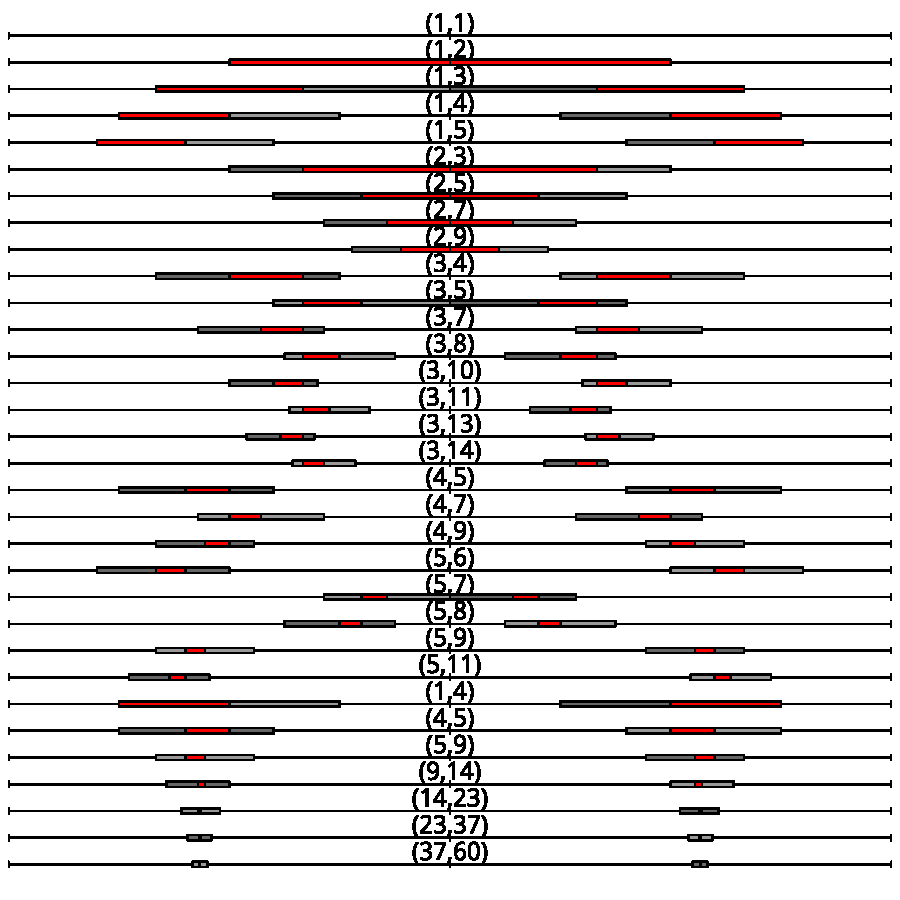
\includegraphics{figdir/fig-gi}
\caption{Generating intervals for a range of parastichy pairs.  Pink: subinterval on which pair is opposed; Light grey: subinterval on which pair is unopposed and $\Delta=+1$;Dark grey: unopposed and $\Delta=-1$. $d=\jhalf$ is not in any generating interval except for $(m,n)=(1,1)$; otherwise $\Delta$ in the opposed subinterval is the same as in the unopposed subintervals}
\label{fig:ogi}
\end{figure}
\end{center}





\end{document}

